% !TEX TS-program = pdflatex
% !TEX encoding = UTF-8 Unicode

% This is a simple template for a LaTeX document using the "article" class.
% See "book", "report", "letter" for other types of document.

\documentclass[11pt]{article} % use larger type; default would be 10pt

\usepackage[utf8]{inputenc} % set input encoding (not needed with XeLaTeX)

%%% Examples of Article customizations
% These packages are optional, depending whether you want the features they provide.
% See the LaTeX Companion or other references for full information.

%%% PAGE DIMENSIONS
\usepackage{geometry} % to change the page dimensions
\geometry{a4paper} % or letterpaper (US) or a5paper or....
% \geometry{margin=2in} % for example, change the margins to 2 inches all round
% \geometry{landscape} % set up the page for landscape
%   read geometry.pdf for detailed page layout information

\usepackage{graphicx} % support the \includegraphics command and options
\usepackage{float}

% \usepackage[parfill]{parskip} % Activate to begin paragraphs with an empty line rather than an indent

%%% PACKAGES
\usepackage{booktabs} % for much better looking tables
\usepackage{array} % for better arrays (eg matrices) in maths
\usepackage{paralist} % very flexible & customisable lists (eg. enumerate/itemize, etc.)
\usepackage{verbatim} % adds environment for commenting out blocks of text & for better verbatim
\usepackage{subfig} % make it possible to include more than one captioned figure/table in a single float
% These packages are all incorporated in the memoir class to one degree or another...

%%% HEADERS & FOOTERS
\usepackage{fancyhdr} % This should be set AFTER setting up the page geometry
\pagestyle{fancy} % options: empty , plain , fancy
\renewcommand{\headrulewidth}{0pt} % customise the layout...
\lhead{}\chead{}\rhead{}
\lfoot{}\cfoot{\thepage}\rfoot{}

%%% SECTION TITLE APPEARANCE
\usepackage{sectsty}
\allsectionsfont{\sffamily\mdseries\upshape} % (See the fntguide.pdf for font help)
% (This matches ConTeXt defaults)

%%% ToC (table of contents) APPEARANCE
\usepackage[nottoc,notlof,notlot]{tocbibind} % Put the bibliography in the ToC
\usepackage[titles,subfigure]{tocloft} % Alter the style of the Table of Contents
\renewcommand{\cftsecfont}{\rmfamily\mdseries\upshape}
\renewcommand{\cftsecpagefont}{\rmfamily\mdseries\upshape} % No bold!

%% Automata
\usepackage{pgf}
\usepackage{tikz}
\usetikzlibrary{arrows,automata,positioning}
\usepackage{tikz-qtree}

%% Rotate text in tables etc.
\def\rot{\rotatebox}

%%% END Article customizations


%%% The "real" document content comes below...

\title{Exercises Compiler Construction}
\author{Martijn Verkleij (s1466895) \& Wouter Bos (s1606824)}
%\date{} % Activate to display a given date or no date (if empty),
         % otherwise the current date is printed 

\begin{document}
\maketitle

\section*{Exercise 8.1}
\begin{tabular}{l|lllllll}
\textit{\textbf{Scope}} & \textit{\textbf{a}}      & \textit{\textbf{b}}      & \textit{\textbf{c}}      & \textit{\textbf{d}}       & \textit{\textbf{e}}       & \textit{\textbf{f}}      & \textit{\textbf{g}}       \\ \hline
\textit{\textbf{Main}}  & \textless1,0\textgreater & \textless1,4\textgreater & \textless1,8\textgreater & \textless1,12\textgreater & \textless1,16\textgreater & -                        & -                         \\
\textit{\textbf{P4}}    & \textless2,0\textgreater & \textless1,4\textgreater & \textless2,4\textgreater & \textless2,12\textgreater & \textless1,16\textgreater & -                        & -\textless2,8\textgreater \\
\textit{\textbf{P1}}    & \textless1,0\textgreater & \textless2,0\textgreater & \textless1,8\textgreater & \textless2,4\textgreater  & \textless1,16\textgreater & \textless2,8\textgreater & -                         \\
\textit{\textbf{P2}}    & \textless1,0\textgreater & \textless2,0\textgreater & \textless1,8\textgreater & \textless2,4\textgreater  & \textless1,16\textgreater & \textless2,8\textgreater & -                         \\
\textit{\textbf{P3}}    & \textless3,0\textgreater & \textless3,4\textgreater & \textless1,8\textgreater & \textless2,4\textgreater  & \textless1,16\textgreater & \textless2,8\textgreater & -                         \\
\textit{\textbf{P5}}    & \textless2,0\textgreater & \textless1,4\textgreater & \textless3,0\textgreater & \textless3,4\textgreater  & \textless1,16\textgreater & -                        & \textless2,8\textgreater 
\end{tabular}

\section*{Exercise 8.2}
\begin{center}
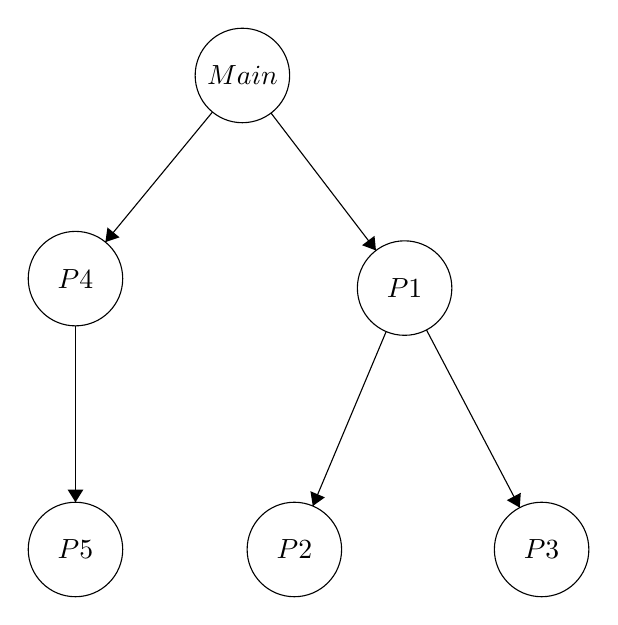
\begin{tikzpicture}[scale=0.2]
\tikzstyle{every node}+=[inner sep=0pt]
\draw [black] (38.7,-5.2) circle (3);
\draw (38.7,-5.2) node {$Main$};
\draw [black] (49,-18.7) circle (3);
\draw (49,-18.7) node {$P1$};
\draw [black] (28.1,-35.3) circle (3);
\draw (28.1,-35.3) node {$P5$};
\draw [black] (42,-35.3) circle (3);
\draw (42,-35.3) node {$P2$};
\draw [black] (57.7,-35.3) circle (3);
\draw (57.7,-35.3) node {$P3$};
\draw [black] (28.1,-18.1) circle (3);
\draw (28.1,-18.1) node {$P4$};
\draw [black] (36.8,-7.52) -- (30,-15.78);
\fill [black] (30,-15.78) -- (30.9,-15.48) -- (30.13,-14.85);
\draw [black] (40.52,-7.59) -- (47.18,-16.31);
\fill [black] (47.18,-16.31) -- (47.09,-15.38) -- (46.3,-15.98);
\draw [black] (28.1,-21.1) -- (28.1,-32.3);
\fill [black] (28.1,-32.3) -- (28.6,-31.5) -- (27.6,-31.5);
\draw [black] (47.83,-21.46) -- (43.17,-32.54);
\fill [black] (43.17,-32.54) -- (43.94,-31.99) -- (43.02,-31.6);
\draw [black] (50.39,-21.36) -- (56.31,-32.64);
\fill [black] (56.31,-32.64) -- (56.38,-31.7) -- (55.49,-32.17);
\end{tikzpicture}
\end{center}

\section*{Exercise 8.3}
\begin{center}
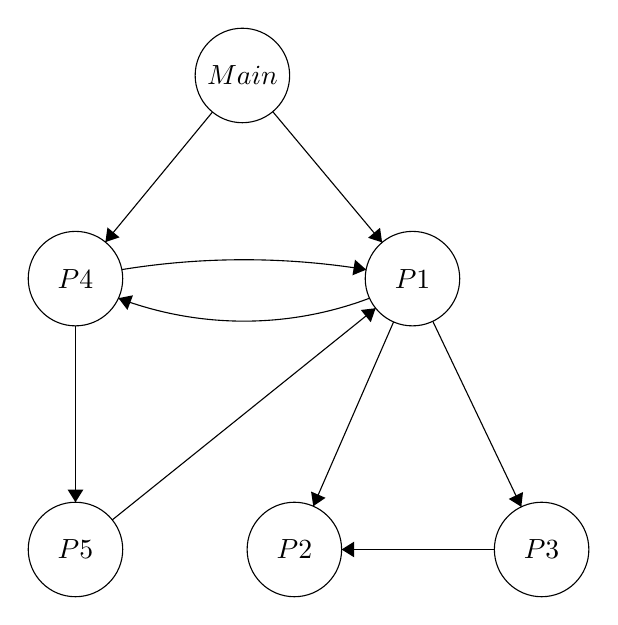
\begin{tikzpicture}[scale=0.2]
\tikzstyle{every node}+=[inner sep=0pt]
\draw [black] (38.7,-5.2) circle (3);
\draw (38.7,-5.2) node {$Main$};
\draw [black] (49.5,-18.1) circle (3);
\draw (49.5,-18.1) node {$P1$};
\draw [black] (28.1,-35.3) circle (3);
\draw (28.1,-35.3) node {$P5$};
\draw [black] (42,-35.3) circle (3);
\draw (42,-35.3) node {$P2$};
\draw [black] (57.7,-35.3) circle (3);
\draw (57.7,-35.3) node {$P3$};
\draw [black] (28.1,-18.1) circle (3);
\draw (28.1,-18.1) node {$P4$};
\draw [black] (36.8,-7.52) -- (30,-15.78);
\fill [black] (30,-15.78) -- (30.9,-15.48) -- (30.13,-14.85);
\draw [black] (40.63,-7.5) -- (47.57,-15.8);
\fill [black] (47.57,-15.8) -- (47.44,-14.87) -- (46.68,-15.51);
\draw [black] (28.1,-21.1) -- (28.1,-32.3);
\fill [black] (28.1,-32.3) -- (28.6,-31.5) -- (27.6,-31.5);
\draw [black] (48.3,-20.85) -- (43.2,-32.55);
\fill [black] (43.2,-32.55) -- (43.98,-32.02) -- (43.06,-31.62);
\draw [black] (50.79,-20.81) -- (56.41,-32.59);
\fill [black] (56.41,-32.59) -- (56.52,-31.65) -- (55.61,-32.09);
\draw [black] (46.773,-19.344) arc (-69.29081:-110.70919:22.545);
\fill [black] (30.83,-19.34) -- (31.4,-20.09) -- (31.75,-19.16);
\draw [black] (31.044,-17.527) arc (99.24266:80.75734:48.288);
\fill [black] (46.56,-17.53) -- (45.85,-16.9) -- (45.69,-17.89);
\draw [black] (30.44,-33.42) -- (47.16,-19.98);
\fill [black] (47.16,-19.98) -- (46.22,-20.09) -- (46.85,-20.87);
\draw [black] (54.7,-35.3) -- (45,-35.3);
\fill [black] (45,-35.3) -- (45.8,-35.8) -- (45.8,-34.8);
\end{tikzpicture}
\end{center}

\section*{Exercise 9}
\begin{figure}[H]
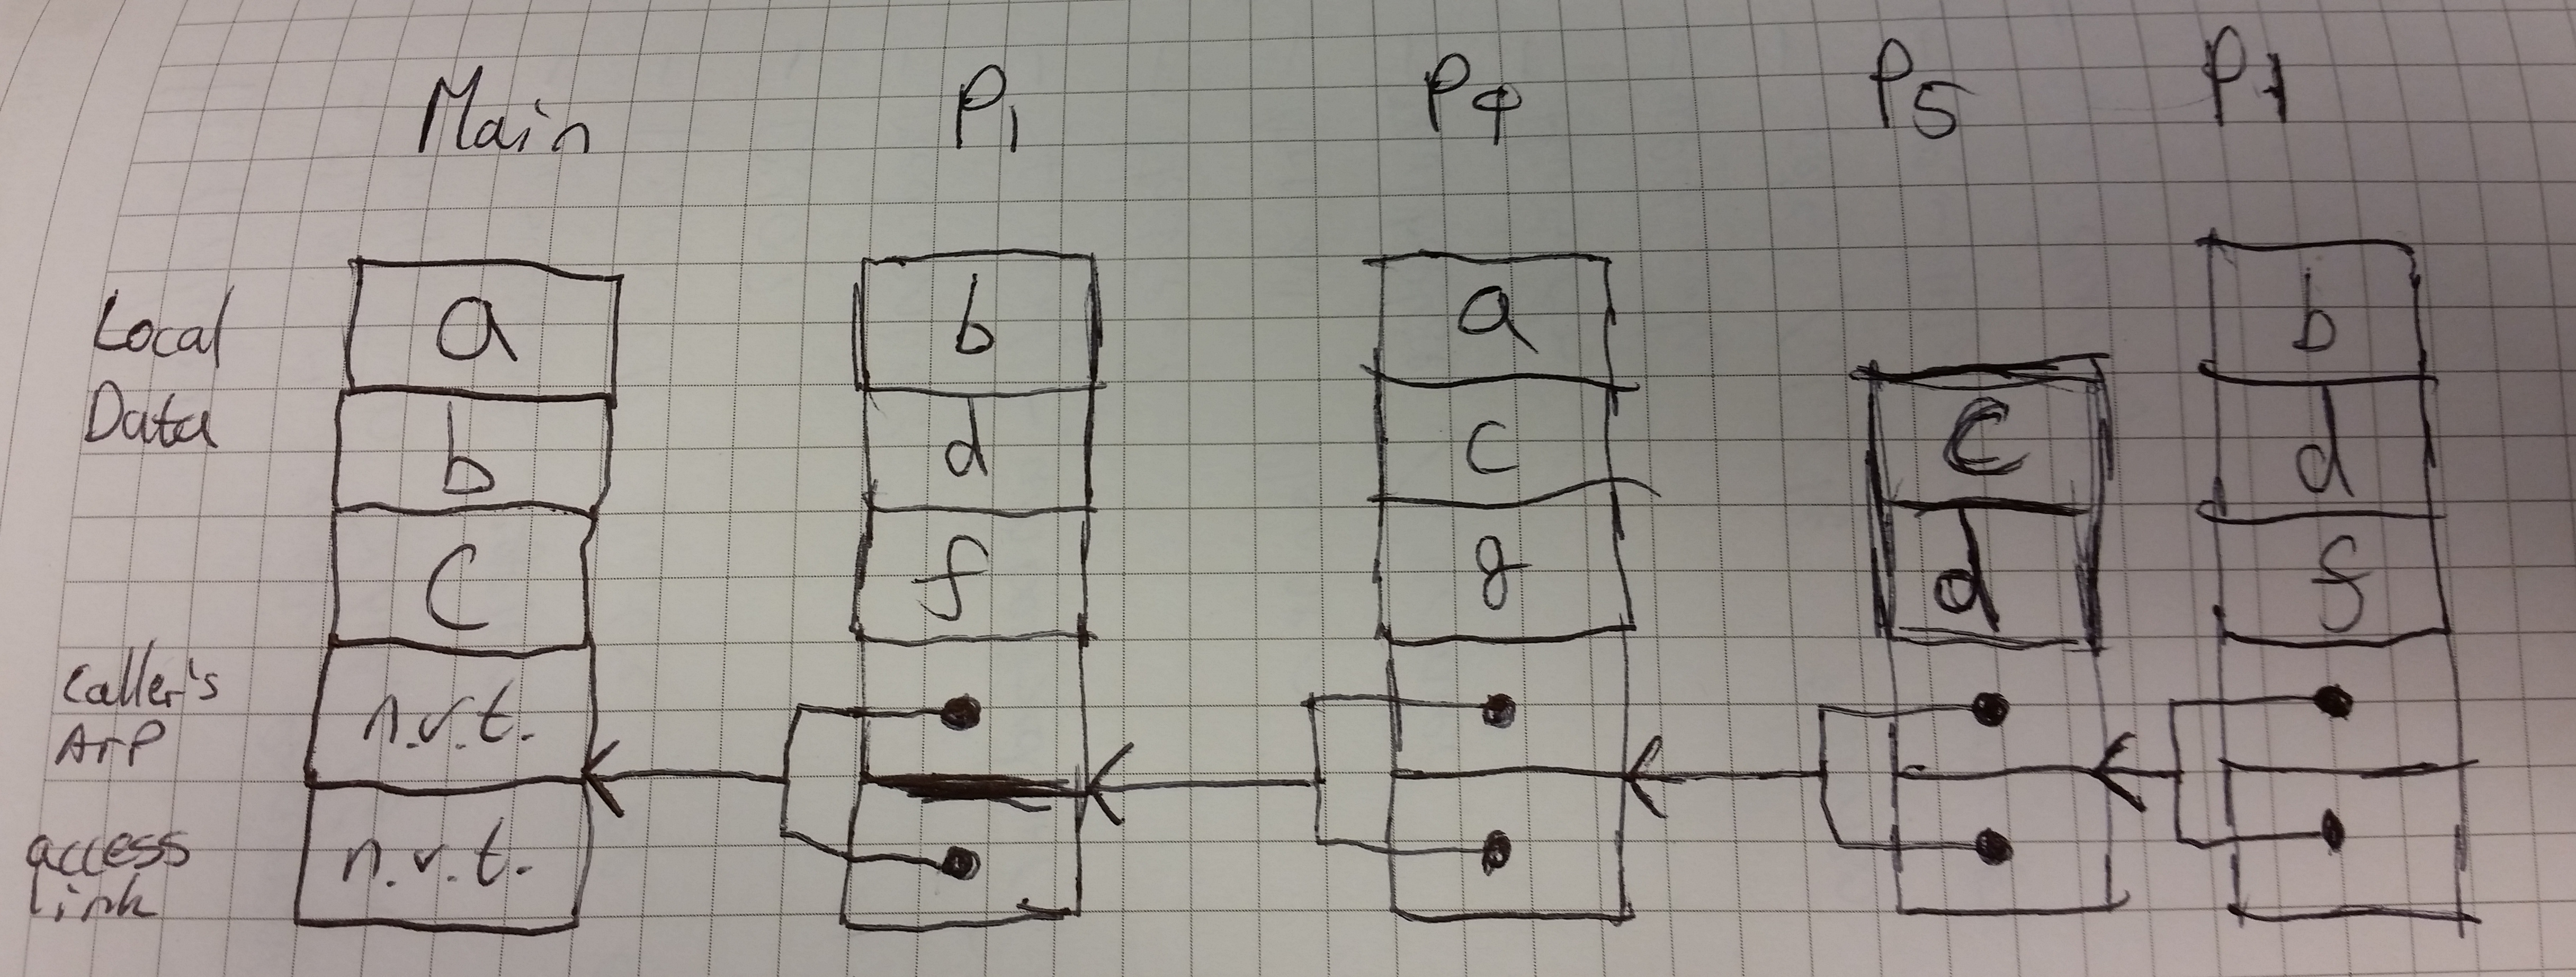
\includegraphics[width=\textwidth]{Ex5-9.jpg}
\caption{The activation records for \texttt{main} [p.304 EC]}
\end{figure}

\section*{Exercise 10}
\begin{figure}[H]
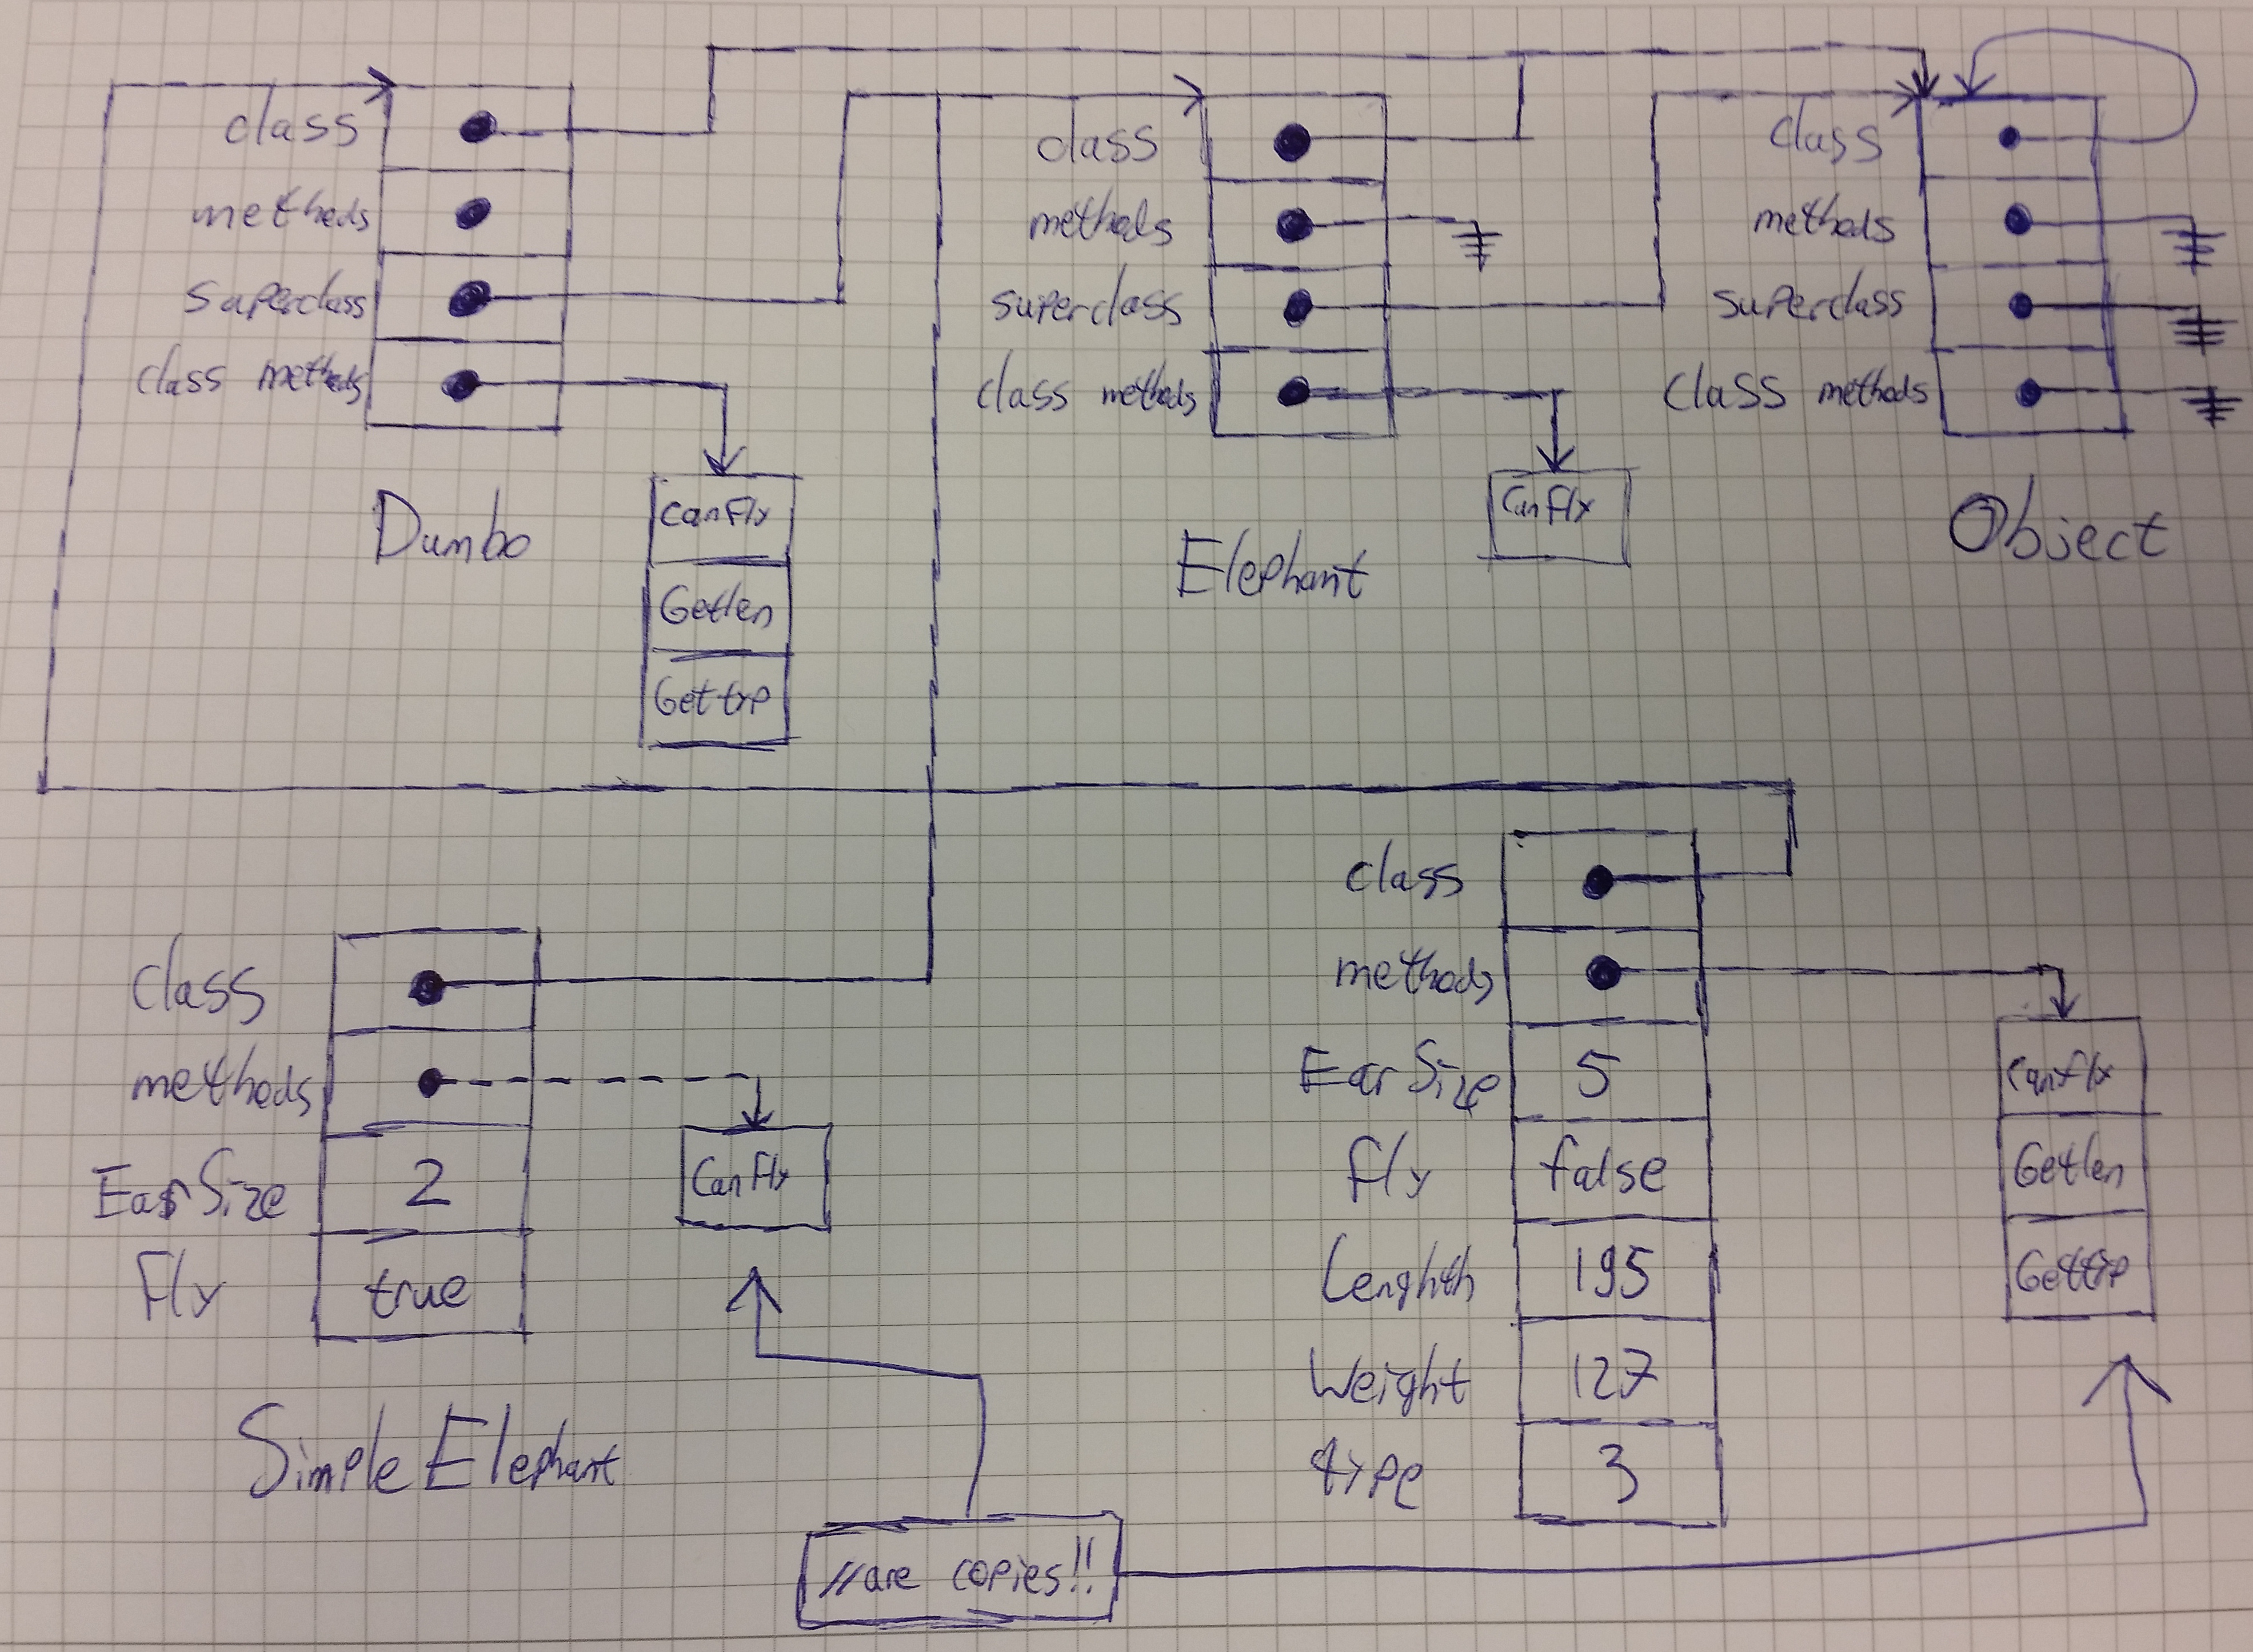
\includegraphics[width=\textwidth]{Ex5-10.jpg}
\caption{The class structure for Dumbo [p.326 EC]}
\end{figure}

\section*{Exercise 11}
\begin{figure}[H]
\centering
\begin{tabular}{ccccc}
line & \multicolumn{3}{c}{\texttt{a}} & \texttt{i} \\ 
\hline 
6 & [1, & 10, & 77] & 1 \\ 
7 & [1, & 5, & 77] & 1 \\ 
8 & [1, & 5, & 77] & 2 \\ 
9 & [1, & 5, & 77] & 2 \\ 
\hline 
\end{tabular} 
\caption{Variable content for call-by-value}
\end{figure}

\begin{figure}[H]
\centering
\begin{tabular}{ccccc}
line & \multicolumn{3}{c}{\texttt{a}} & \texttt{i} \\ 
\hline 
6 & [1, & 13, & 77] & 1 \\ 
7 & [1, & 5, & 77] & 1 \\ 
8 & [1, & 5, & 77] & 2 \\ 
9 & [1, & 9, & 77] & 2 \\ 
\hline 
\end{tabular} 
\caption{Variable content for call-by-reference}
\end{figure}

\begin{figure}[H]
\centering
\begin{tabular}{ccccc}
line & \multicolumn{3}{c}{\texttt{a}} & \texttt{i} \\ 
\hline 
6 & [1, & 13, & 77] & 1 \\ 
7 & [1, & 5, & 77] & 1 \\ 
8 & [1, & 5, & 77] & 2 \\ 
9 & [1, & 5, & 81] & 2 \\ 
\hline 
\end{tabular} 
\caption{Variable content for call-by-name}
\end{figure}

\section*{Exercise 12}
\begin{figure}[H]
\centering
\begin{tabular}{|c|}
\hline 
Access Link(2) \\ 
Return Address(6) \\ 
b \\ 
\hline 
a \\ 
Access Link(14) \\ 
Return Address (19) \\ 
g \\ 
\hline 
a \\ 
Access Link(8) \\ 
Return Address (23) \\
\hline
a \\ 
Access Link (1) \\ 
Return Address (26) \\ 
\hline
Access Link (0) \\ 
Return Address (0) \\ 
\hline 
\end{tabular} 
\caption{Variable content for call-by-name}
\end{figure}

\section*{Exercise 12}

\begin{itemize}
\item \texttt{x}: Callee saves, the caller knows that it still needs the value, but callees may be able to determine they do not need the register and therefore do not need to save the register in memory.
\item \texttt{a and c}: Caller saves, the caller knows that it still needs the value, but a lot of calls are still happening, so a great chance exists that values will be overwritten.
\end{itemize}
\end{document}


